%% Template for a preprint Letter or Article for submission
%% to the journal Nature.
%% Written by Peter Czoschke, 26 February 2004
%%

\documentclass{nature}
%\documentclass[12pt]{article}

%% make sure you have the nature.cls and naturemag.bst files where
%% LaTeX can find them

\bibliographystyle{naturemag}

\usepackage{graphicx}
\usepackage{amssymb,amsfonts,amsmath}
\usepackage{subfigure}
\usepackage{stfloats}


%% OPTIONAL MACRO DEFINITIONS
\def\s{\sigma}
\newcommand{\be}[0]{\begin{equation}}
\newcommand{\ee}[0]{\end{equation}}
\newcommand{\lb}[0]{\left(}
\newcommand{\rb}[0]{\right)}


\title{Human-induced Arctic sea-ice loss and cold Eurasian winters}

%% Notice placement of commas and superscripts and use of &
%% in the author list


\author{K. E. McCusker*$^{1,2}$, \& John C. Fyfe,$^{2}$, \& Michael Sigmond$^2$}

% NatGeo requirements:
% Title If possible, the title should give a sense of the main new finding, and should not exceed 90 characters, including spaces. Nature Geoscience titles do not contain technical terms or abbreviations unless absolutely necessary. We strongly discourage punctuation or active verbs.@@
% Letter 2,000 words no methods, 3 figures
% Article 3,000 words no methods, include section titles, 6 figures. No refs in abstract. ~500 words of Intro. 1-2 para of conclusions


\begin{document}

\maketitle

\begin{affiliations}
 \item School of Earth and Ocean Sciences, University of Victoria, Victoria, BC, V8P 5C2, Canada
 \item Canadian Centre for Climate Modelling and Analysis, Environment Canada, Victoria, BC V8W 2Y2, Canada
\end{affiliations}


\begin{abstract}
Arctic sea ice loss has been implicated in the recent trend toward unusually cold Eurasian winters \cite{liu12,mori14,kim14}. Whether the linkage follows from anthropogenic sea ice loss, however, remains an open question as the sea-ice loss combines anthropogenic response and internal (random) variability \cite{swart15,wettstein14} and because of confounding wintertime variability over the Eurasian continent \cite{deser12b,screen14a}. Here, we isolate the anthropogenic and random components of the linkage using a large ensemble of atmosphere-only model simulations with prescribed sea ice loss taken from simulations of the companion atmosphere-ocean-cryosphere model. We find no evidence of a sea-ice loss related decrease in Eurasian winter temperature. However, we do find long periods of winter Eurasian cooling linked to internally-generated circulation features over the Barents and Kara Seas regions of the Arctic. These results challenge the perception that Arctic sea ice loss was responsible for the recent prevalence of unusually cold Eurasian winters, showing instead that these winters were more likely the consequence of internal variability, with implications for our understanding of impacts and adaptation in human and natural high-northern latitude systems. %We find no evidence of a sea-ice loss related increase in the prevalence of cold Eurasian winters.
\end{abstract}

Average northern hemisphere winter (Dec-Feb; DJF) temperature has increased @@ $^\circ$C/decade since 1979. The majority of this warming is attributed to anthropogenic greenhouse gas emissions (@@cite) combined with positive feedbacks related to the loss of Arctic sea ice (@@cite). Epoch differences of surface air temperature (SAT) between 2002-12 and 1979-89 reveal warming upwards of 2$^\circ$C over the polar cap, collocated with areas of sea ice loss (Figure \ref{fig:fig1}a). Contemporaneous cooling of greater than 1$^\circ$C over the Eurasian continent in winter is striking against this general hemispheric warming. Figure \ref{fig:fig1}b shows that in the 11 years from 2002-12, 7 of the 10 coldest Eurasian winters occurred

, as it must overcome a significant anthropogenically forced warming signal. 



\begin{methods}
\textbf{Observations} \\
blah blah blah
\\
\textbf{Model simulations}\\
blah
\end{methods}

\begin{figure}%[htbp] % the star afterwards makes it a one column fig in a 2-col document
\centering
\noindent\includegraphics[width=19pc]{Figure1.pdf}
\caption{\textbf{Observed surface air temperature and sea ice concentration. Open circle markers indicate regions of sea ice loss (red) and gain (blue) that are greater than 40\% in absolute terms.} 
}
\label{fig:fig1} 
\end{figure}

\begin{figure}%[htbp] % the star afterwards makes it a one column fig in a 2-col document
\centering
\noindent\includegraphics[width=19pc]{Figure2.pdf}
\caption{\textbf{CanESM2 large ensemble change in winter sea ice area.} 
}
\label{fig:fig2} 
\end{figure}

\begin{figure}%[htbp] % the star afterwards makes it a one column fig in a 2-col document
\centering
\noindent\includegraphics[width=35pc]{Figure3.pdf}
\caption{\textbf{Polar cap and Eurasian temperature response uncertainty cascades.} 
}
\label{fig:fig3} 
\end{figure}

\begin{figure}%[htbp] % the star afterwards makes it a one column fig in a 2-col document
\centering
\noindent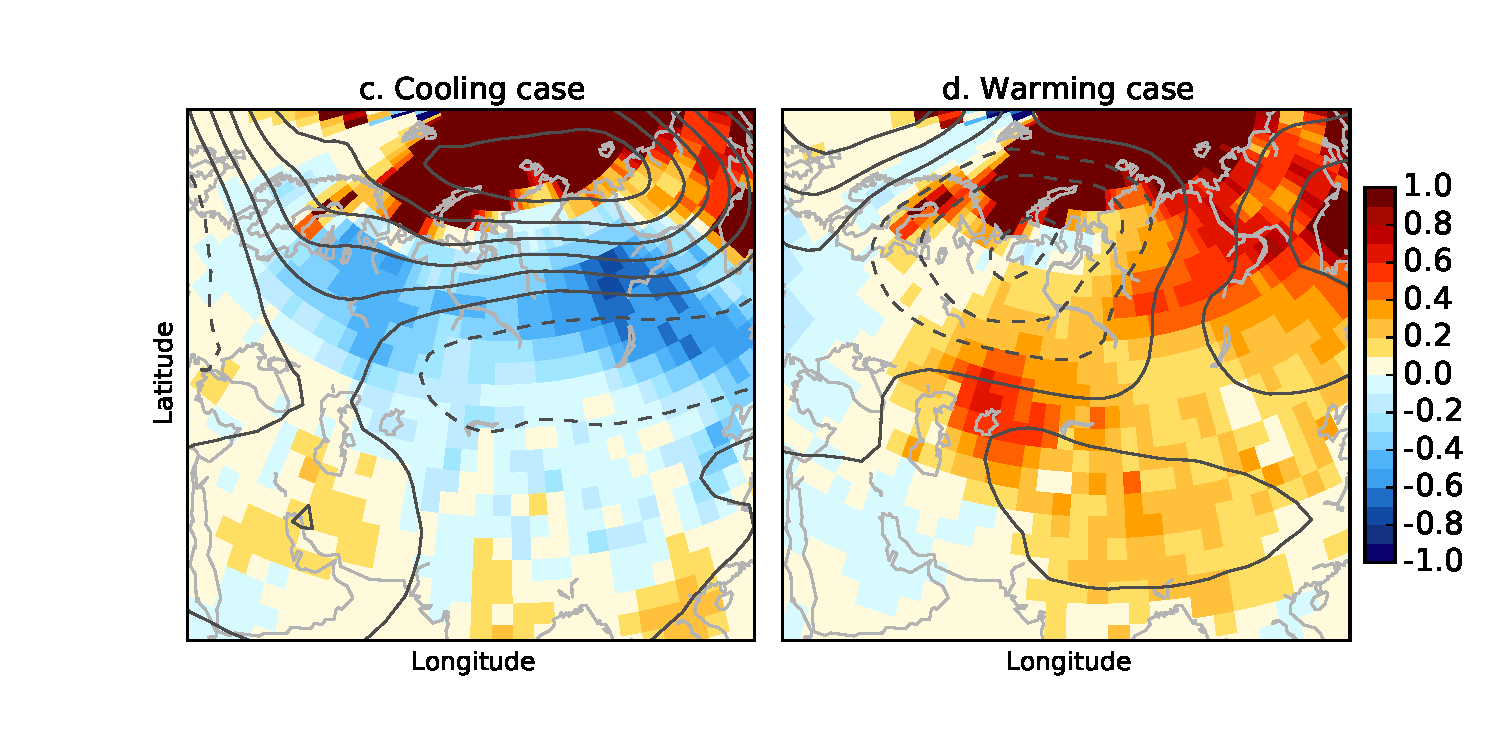
\includegraphics[width=39pc]{Figure4_orSuppFig2.pdf}
\caption{\textbf{Winter surface air temperature and geopotential height responses.} 
}
\label{fig:fig4} 
\end{figure}

\begin{figure}%[htbp] % the star afterwards makes it a one column fig in a 2-col document
\centering
\noindent\includegraphics[width=19pc]{Figure5_draft.pdf}
\caption{\textbf{Winter Eurasian surface air temperature versus Barents-Kara geopotential height.} 
}
\label{fig:fig5} 
\end{figure}


%% Put the bibliography here, most people will use BiBTeX in
%% which case the environment below should be replaced with
%% the \bibliography{} command.

%\begin{thebibliography}{1}
%\end{thebibliography}
\newpage

%\bibliographystyle{ametsoc}
\bibliography{allrefs}





% ~/bibtexrefs/allrefs  == this is version controlled now, but will have to just copy into current dir?


%% Here is the endmatter stuff: Supplementary Info, etc.
%% Use \item's to separate, default label is "Acknowledgements"

\begin{addendum}
\item[Acknowledgements] 
\item[Author Contributions] 
 \item[Competing Interests] The authors declare that they have no competing financial interests.
\item[Correspondence] Correspondence and requests for materials should be addressed to K.E.M.~(email: kemccusk@uvic.ca).
\end{addendum}

%%
%% TABLES
%%
%% If there are any tables, put them here.
%%

\end{document}
